% Generated by scripts/build-paper.py — edit paper/src/survey.src.md
\section{Evidence synthesis}\label{sec:evidence-synthesis}

\subsection{The evidence base}

The core studies appeared between 19 September and 6 October 2026, beginning four days after the launch (Figure 1). Relationships overlap: 61 studies evaluate hosted Jev, 52 build or evaluate independent Jev-like models, and 20 embed typed decisions in a larger system (Table 3). In all, 75 studies call hosted Jev, as the object of study, a baseline or a component; 63 state the version they called and 12 state none. Every core study is an arXiv preprint.

\begin{figure}[tbp]
\centering
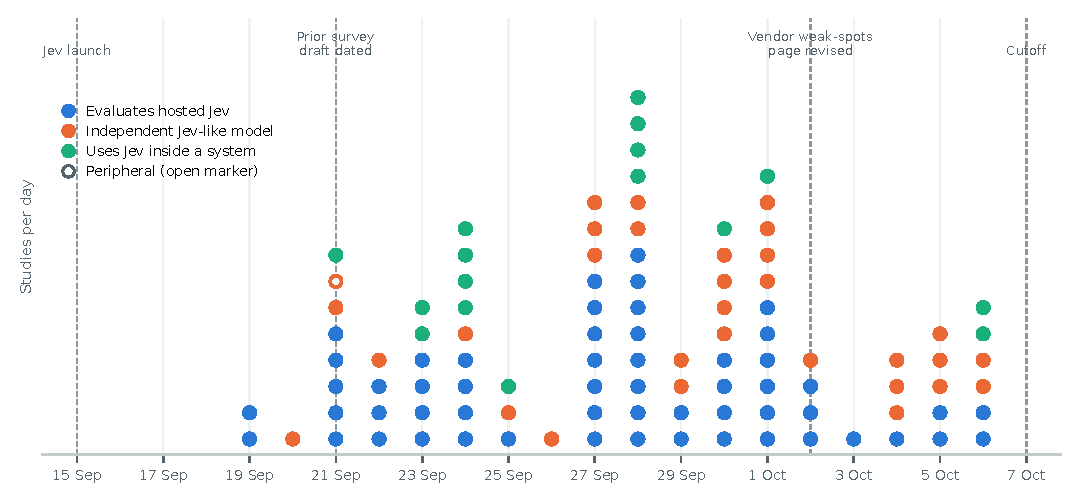
\includegraphics[width=\linewidth]{figures/timeline.pdf}
\caption{Submission dates (arXiv v1) of the core and peripheral studies, one dot per study stacked by day and coloured by primary relationship to Jev, against context events.}\label{fig:timeline}
\end{figure}

{\footnotesize
\begin{xltabular}{\linewidth}{p{0.2\linewidth}p{0.055\linewidth}p{0.085\linewidth}p{0.11\linewidth}Xp{0.075\linewidth}}
\caption{Core and peripheral studies (* peripheral; † same study family). Headline values are author-reported.}\label{tab:core}\\
\toprule
\textbf{Study} & \textbf{v1 (2026)} & \textbf{Test level} & \textbf{Version} & \textbf{Headline (as reported)} & \textbf{Ref.} \\
\midrule
\endfirsthead
\toprule
\textbf{Study} & \textbf{v1 (2026)} & \textbf{Test level} & \textbf{Version} & \textbf{Headline (as reported)} & \textbf{Ref.} \\
\midrule
\endhead
Replacing LLMs with Jev at the Edge † & 09-19 & Hybrid & jev-1.13.0 & Median decision latency −22.7\% to −64.5\% vs the fastest LLM & \citep{arxiv2609_22753} \\
Intent at RIC Timescales † & 09-19 & Hybrid & jev-1.13.0 & Meets the 1 s RIC budget on 99.8\% of calls (LLMs: 17.9\%, 0\%) & \citep{arxiv2609_23136} \\
this-that-model-1.0 & 09-20 & Model test & 1.0; not reported & 30.9 ms per decision on one laptop GPU; 32 decisions/\allowbreak{}s & \citep{arxiv2609_23886} \\
Open-Jev on CallScreenBench & 09-21 & Model test & paper v1 (three seeds) & JevLite ensemble AUROC .974, ECE .052; no false alarms & \citep{arxiv2609_23959} \\
Jev-Mem & 09-21 & System test & not reported & LoCoMo judge 0.777 (+11.0\%); build 158 s; 0.93 s/\allowbreak{}query & \citep{arxiv2609_23986} \\
Calibrated Decisions at Scale † & 09-21 & System test & jev-1.13.0 & 499,500 narratives screened for \$25.23; 195,857 fully coded & \citep{arxiv2609_24052} \\
JEVQA & 09-21 & Model test & jev-1.13 & PLCC vs VMAF: 0.737 (metadata) → 0.824 (+bitstream, pixel) & \citep{arxiv2609_24395} \\
Decision Models for CSS Annotation & 09-21 & Model test & typesafe/\allowbreak{}jev1.13 & Behind best LLM on 14/\allowbreak{}15 tasks (−11.6 F1) at 44× lower cost & \citep{arxiv2609_24574} \\
Pregnancy in Crash Narratives † & 09-21 & Model test & jev-1.13.0 & Population-scale reading audited by blind coders: sensitivity 0.999 & \citep{arxiv2610_00213} \\
Jev for Scientific Decisions & 09-21 & System test & Jev 1.13 & Full semantic correctness; median 0.335 s, p95 0.442 s & \citep{arxiv2609_24965} \\
Universal Fractal Decision Map * & 09-21 & Model test & not reported & Self-reported 81.65\% on public JevBench items at 7.08 ms & \citep{arxiv2609_25498} \\
Visual Jev & 09-22 & Model test & paper v1 & Macro accuracy 0.706 → 0.761 after post-training (seen families) & \citep{arxiv2609_25845} \\
REFLEX with Jev † & 09-22 & System test & jev-1.13.0 & 95\% success with 1.12 strong calls/\allowbreak{}task vs 88\% and 4.10 (−72.7\%) & \citep{arxiv2609_26532} \\
JEV-as-a-Judge & 09-22 & Model test & jev-1.13.0 & Within 3 points of GPT-6 where the verdict can be read off the text & \citep{arxiv2609_26550} \\
Type-Safe Is Not Error-Free & 09-22 & Model test & not reported & Hosted Jev AUROC .8146 → .5806 after name–rubric swap; 0\% type errors & \citep{arxiv2609_26758} \\
JEV-Star & 09-23 & System test & Jev 1.13 & 4/\allowbreak{}4 full-game wins incl. two vs Lv7 with GPT-6 plans; Jev-only never expanded & \citep{arxiv2609_27331} \\
KITE & 09-23 & System test & jev-1.13.0 & 1.7\% flagship anchors cut effect error 41\%; decision gain 0.27 → 0.39 & \citep{arxiv2609_27535} \\
Jev as a Radiology Report Judge & 09-23 & Model test & jev-1.13.0 & Kendall τ 0.573 /\allowbreak{} 0.398 with expert error counts; beats open NLI & \citep{arxiv2609_27607} \\
Jev on Contract Inference & 09-23 & Model test & jev-1.13.0 & \$0.000228 and 1.24 s per contract — lowest of ten models & \citep{arxiv2609_27678} \\
NumericJev & 09-23 & Model test & jev-1.13 & Range refinement: 83.4\% within 5\% vs 80.5\% direct choice & \citep{arxiv2609_28587} \\
Decision Hijacking † & 09-23 & Model test & jev-1.13.0 & Injection shifts probabilities (+0.043) but rarely selects the target (1.8\%) & \citep{arxiv2609_28613} \\
Harness Tokenomics & 09-24 & Simulation & jev-1.13.0 & Emulated router saves 13–21\% of coding-agent spend & \citep{arxiv2609_28919} \\
Pentest Decision Layers & 09-24 & System test & jev-latest & One run each: 5 min faster, different severities — not a controlled test & \citep{arxiv2609_28940} \\
PixelJev † & 09-24 & Model test & — & Typed readout and generation gain equally after adaptation & \citep{arxiv2609_29283} \\
Just Ask Jev & 09-24 & Model test & jev-1.13.0 & Zero-shot failure detection: median AUROC 0.886 at 1/\allowbreak{}63 of judge cost & \citep{arxiv2609_29429} \\
Jev as a Rubric Judge & 09-24 & Model test & jev-1.13.0 & Parity on most rubric criteria at 1/\allowbreak{}16–1/\allowbreak{}325 of the cost & \citep{arxiv2609_29769} \\
Jev-Mobile & 09-24 & System test & not reported & AndroidWorld 79\% (vs 84\% step-wise) at 73\% lower API cost & \citep{arxiv2609_30186} \\
Jev in the Wild & 09-24 & Not applicable & not reported & Ecosystem: judgment 77\%, scoring 52\%, action selection 31\% of projects & \citep{arxiv2609_30216} \\
JevOut & 09-24 & Model test & jev-1.13.0 & Natural context flips 61\% of correct decisions (vs 2\% neutral) & \citep{arxiv2609_30243} \\
Biosecurity Audit & 09-24 & Model test & jev-1.13.0 & Confidence = chance-normalised max probability; pooled ECE 0.034 & \citep{arxiv2609_30454} \\
LAVOIR & 09-25 & Model test & — & Learned “when to ask” policy ≈ oracle (AUC 0.80 vs 0.80) & \citep{arxiv2609_30706} \\
JevSoup & 09-25 & System test & jev-1.13.0 & Jev-routed LoRA composition: +0.2 to +1.2 points & \citep{arxiv2609_30922} \\
JevAdvBench & 09-25 & Model test & jev-1.13.0 & An appended opinion flips 12\% and drains 38\% of confident answers below the gate & \citep{arxiv2609_31142} \\
PACT & 09-26 & Model test & — & Open recipe holds up; extra terms buy robustness, not accuracy & \citep{arxiv2609_35865} \\
Probability Axioms & 09-27 & Model test & jev-1.13 & P(X) + P(not X) misses 1 by 0.064 (open LLM readout: 0.293) & \citep{arxiv2609_33209} \\
Agent Security Decisions & 09-27 & Model test & jev-1.13 & Safe automation coverage: 7.6\% (symmetric) → 47\% (separate thresholds) & \citep{arxiv2609_33401} \\
Speech Neuroprosthesis Rescoring & 09-27 & Model test & jev-latest & Rescoring: WER 7.5\% vs 7.8\% for 7B LLMs, no GPU needed & \citep{arxiv2609_33538} \\
COGNIT-Guard & 09-27 & Model test & — & Adapted open guard: AUC 0.83 → 0.997, with an OOD “alignment tax” & \citep{arxiv2609_33671} \\
Typed Decisions for 5G Control & 09-27 & System test & jev-1.13.0 & Hosted Jev never meets 100 ms near-RT deadlines (warm p50 281 ms) & \citep{arxiv2609_33689} \\
Laya Reproduction † & 09-27 & Model test & — & Open Laya checkpoint under-confident (gap −0.214); one temperature fixes it & \citep{arxiv2609_33843} \\
Probability Contracts & 09-27 & Model test & jev-1.13.0 & Two interfaces, same question: different decision on 32.8\% of pairs & \citep{arxiv2609_37470} \\
JET & 09-27 & Model test & Jev 1.13 & Local likelihood readout 85.1\% vs Jev 89.1\% on MMLU & \citep{arxiv2609_33874} \\
Do Decisions Add Up? & 09-27 & Model test & jev-1.13.0 & Staged decisions disagree with direct ones; Jev loses 22.9 points on CLINC150 & \citep{arxiv2609_33971} \\
Jev in Medicine & 09-27 & Model test & jev-1.13 & Medicine: parity on abstracts, −22 points on diagnostic cases & \citep{arxiv2609_34024} \\
Video Anomaly Readouts & 09-28 & Model test & jev-1.13.0 & Same evidence, different readout: +18 AP on one dataset, none on the other & \citep{arxiv2609_34180} \\
Selection vs Extraction Memory & 09-28 & System test & jev-1.13.0 & One Jev selection call ≈ LLM-extraction memory at 1/\allowbreak{}3,061 the write cost & \citep{arxiv2609_34227} \\
SeLMRoute & 09-28 & System test & not reported & Typed-question features route LLMs: 72.1\% vs 69.2\% best single model & \citep{arxiv2609_34736} \\
Agent Trace Security Judge & 09-28 & Model test & not reported & Trace security: F1 77.8 vs 74.1 for the best LLM judge & \citep{arxiv2609_34862} \\
JevVibe & 09-28 & Model test & jev-1.13.0 & CWE triage: Top-1 0.46 vs 0.50 (frontier) at 1/\allowbreak{}56 of the cost & \citep{arxiv2609_34963} \\
NavJev & 09-28 & System test & not reported & Navigation: 27\% SR at 0.65 s/\allowbreak{}step; components, not just Jev, carry the gain & \citep{arxiv2609_34969} \\
Source-Position Coherence & 09-28 & Model test & jev-1.13.0 & Jev’s argument scores move with the stated source & \citep{arxiv2609_35286} \\
Decide, Don’t Generate (ABSA) & 09-28 & Model test & jev-1.13.0 & SemEval ABSA: best regression error with 488 fitted coefficients & \citep{arxiv2609_35293} \\
Sys1Cal-v1 & 09-28 & Model test & not reported & Known-probability test: Noul 0.92, Score 0.89, Choice 0.76 & \citep{arxiv2609_35342} \\
Mnemon & 09-28 & System test & jev-1.13 & Memory agent: LoCoMo 91.7\% with Jev judging evidence (AUC 0.94) & \citep{arxiv2609_36059} \\
Koa-action & 09-28 & Model test & — & Single-token LLM classifier: 85.5\% at 0.53 s, flat across label spaces & \citep{arxiv2609_36115} \\
Dyad & 09-28 & Model test & Jev 1.13 & Native typed-decision head: 86.2\% vs Jev 85.0\% on JevBench & \citep{arxiv2609_36116} \\
Training-Free HAR & 09-28 & Model test & jev-1.13.0 & Sensor activity recognition from text: macro-F1 ≤ 0.12 & \citep{arxiv2609_36154} \\
Cultural Values Audit & 09-28 & Model test & jev-1.13.0 & Persona shifts reproduce 87\% (English) vs 62\% (Arabic) of a human difference & \citep{arxiv2609_36399} \\
Chinese-Jev & 09-29 & Model test & not reported & Language-specific open encoder ≈ hosted Jev in Chinese, better calibrated & \citep{arxiv2609_36965} \\
Benchmarking Jev (37 datasets) & 09-29 & Model test & jev-1.13.0 & Ahead of a 27B open LLM on 27/\allowbreak{}37 datasets; pooled Choice ECE 0.028 & \citep{arxiv2609_37647} \\
Certo (Cacheable Rules) & 09-29 & Model test & — & Cacheable scoring loses rule sensitivity (recall@1 1.00 → 0.24) & \citep{arxiv2609_37832} \\
Decision Gates Benchmark † & 09-29 & Model test & jev-1.13.0 & Threshold for 5\% risk still admits 31\% of out-of-scope requests & \citep{arxiv2610_00346} \\
Ordinal-Scale Bias & 09-30 & Model test & typesafe/\allowbreak{}jev-1.13-20260917 & ANLI: Neutral absorbs 51\% of errors, at every position & \citep{arxiv2609_38827} \\
OpenJev-RLCD & 09-30 & Model test & — & Open RLCD: best selective prediction among SFT, STaR, GRPO & \citep{arxiv2609_38850} \\
Bongard & 09-30 & Model test & — & Open encoder–decoder: 78.05\% on DecisionBench, 32 questions in 221 ms & \citep{arxiv2609_39111} \\
Network Traffic Classification & 09-30 & Model test & typesafe/\allowbreak{}jev-1.13-20260917 & Packet numbers in, 28\% accuracy out — trees trained on 8k records reach 70\% & \citep{arxiv2610_00376} \\
OmniMed-Jev & 09-30 & Model test & — & Same backbone, decision-native output: calibration error down up to 10× & \citep{arxiv2610_00381} \\
Rejection Bottleneck & 09-30 & Model test & jev-1.13 & Present 99\%, rejected when absent 7\% — though Boolean checks get 99\% & \citep{arxiv2609_39496} \\
JevSpawn & 09-30 & System test & jev-1.13.0 & Agent with spawned finite actions: Maze 0.96 vs 0.52 & \citep{arxiv2610_00437} \\
Recommendation Reranking & 09-30 & Model test & jev-latest & Strong reranking quality; latency between local models and pointwise LLMs & \citep{arxiv2609_40241} \\
AnyJev & 09-30 & Model test & — & Order flips on a third of 20-option items; rotation averaging halves them & \citep{arxiv2610_00831} \\
Beyond Answer Confidence & 10-01 & Model test & jev-1.13.0 & Confidence ≠ knowing: +0.21–0.33 overconfidence past the knowledge boundary & \citep{arxiv2610_01006} \\
Jev-IDS & 10-01 & Model test & jev-1.13.0 & Intrusion pilot: F1 0.859, 4.8× faster than an LLM & \citep{arxiv2610_01079} \\
Fast Models, Slow Evidence & 10-01 & Model test & jev-1.13.0 & Hosted beats open on 9 of 11 harness decisions; routing at chance for both & \citep{arxiv2610_02267} \\
Candidate-Independent Attention & 10-01 & Model test & — & Isolate candidates: order flips 18.2\% → 1.2\% & \citep{arxiv2610_01601} \\
Code Owns the Simulation & 10-01 & System test & jev-1.13.0 & Evaluates what is described; does not simulate what is not & \citep{arxiv2610_01834} \\
HakemBench † & 10-01 & Model test & jev-1.13 & Turkish typed decisions: Jev fourth of 16 at a tenth of the leader’s time & \citep{arxiv2610_02293} \\
JEVDB & 10-01 & System test & jev-1.13.0 & Semantic SQL: pruning + typed decisions finish 540K-pair joins & \citep{arxiv2610_02046} \\
HydroJEV & 10-01 & Model test & jev-1.13.0 & Pre-registered gate: a third of SCADA reviews offloaded, accuracy kept & \citep{arxiv2610_02048} \\
LLM-as-Jev & 10-01 & Model test & — & A frozen 4B LLM already matches community Jev-style models & \citep{arxiv2610_02076} \\
SBERT2S1 & 10-01 & Model test & — & Open RLCD recipe trails plain cross-entropy by 2.5–3.0 points & \citep{arxiv2610_02486} \\
Labels Override Definitions & 10-01 & Model test & — & The label wins over the definition — and the cause is one rendering line & \citep{arxiv2610_02586} \\
SecJev & 10-02 & Model test & — & Security-specialised 0.8B beats general 9B by 20.5 points & \citep{arxiv2610_03073} \\
HateDecide & 10-02 & Model test & jev-1.13.0 & Definitions move 28\% of answers — without reliably improving them & \citep{arxiv2610_03324} \\
Candidate Coverage and Transfer & 10-02 & Model test & jev-1.13.0 & Rejection thresholds do not travel: 69\% false rejection after transfer & \citep{arxiv2610_03387} \\
JEVal and InnerJev & 10-02 & Model test & jev-1.13.0 & Right mode, wrong mass: 89\% placed where the truth is 36\% & \citep{arxiv2610_03935} \\
Wireless Decision-Making & 10-03 & Model test & not reported & Wireless control: 3.5–8.5× faster than LLMs; quality depends on the task & \citep{arxiv2610_04345} \\
Hidden Risks of Jev & 10-04 & Model test & not reported & Typed outputs, hijacked inputs: up to 100\% injection success & \citep{arxiv2610_04985} \\
CrystalJev & 10-04 & Model test & — & One calibrated pass against a relaxation: as good or better at a thirtieth of the cost & \citep{arxiv2610_06985} \\
SearchJev & 10-04 & Model test & jev-1.13.0 & Task-specialised open model beats Jev on rewriting, trails on routing & \citep{arxiv2610_05107} \\
Fiorillo & 10-04 & Model test & — & Registered test passed: ECE 0.017, macro-F1 0.92 against 0.87 for a 31B model & \citep{arxiv2610_07019} \\
GraphDecide † & 10-05 & Model test & jev-1.13.0 & Reads every edge; counts degree right 68\% of the time & \citep{arxiv2610_06354} \\
Political Science Replications & 10-05 & Model test & typesafe/\allowbreak{}jev-1.13-20260917 & Same accuracy, no cost advantage at batch prices & \citep{arxiv2610_06625} \\
ufakzeka-karar † & 10-05 & Model test & — & Order invariance by construction; sequential heads still flip 2–3\% & \citep{arxiv2610_06744} \\
CLM-as-a-Judge † & 10-05 & Model test & — & Open contrastive decision model judges near chance, but ignores answer order & \citep{arxiv2610_07177} \\
SharedKV-BT & 10-05 & System test & — & Node-local candidates: 113/\allowbreak{}120 correct decisions against 90/\allowbreak{}120 & \citep{arxiv2610_07327} \\
Readout Stability & 10-06 & Model test & not reported & Menu changes are predictable offline for decision models, not for generative LLMs & \citep{arxiv2610_07716} \\
SanSi & 10-06 & Model test & jev-1.13.0 & Looping a small decision model: +13.5 points at 7.7× compute & \citep{arxiv2610_07730} \\
System One Moderation & 10-06 & Model test & jev-1.13 & Precedents help Jev pick the right rule (+5 to +22 points); Laya barely moves & \citep{arxiv2610_07953} \\
Plans Change Answers & 10-06 & Simulation & — & Calibrated confidence prices query plans; overconfidence hides output errors & \citep{arxiv2610_08089} \\
S1-MAS & 10-06 & System test & — & Laya coordinates agents with 78–94\% fewer GPT tokens; random choices trail by 1.8 points & \citep{arxiv2610_08155} \\
BOTTLED & 10-06 & Model test & jev-1.13.0 & Agent-built artifacts: 94–97\% of Jev’s quality at 2–25\% of its projected cost & \citep{arxiv2610_08775} \\
\bottomrule
\end{xltabular}}

\subsection{F1 · A type-valid answer can still be the wrong answer}

Typed interfaces remove parse and schema failures by construction; they do not make the chosen option right. The most direct test held question, state, rubric wording and the set of option names fixed and changed only which name was bound to which rubric \citep{arxiv2609_26758}. For hosted Jev, rebinding the rubrics behind \emph{no/yes} flipped 32.50\% of answers against about 2\% under neutral names, 24× the model's test–retest floor, and lowered AUROC from .8146 to .5806 while the type-error rate stayed at 0\%. Swapping the meaning of yes and no flipped about half of Jev's answers in a decision-gate benchmark \citep{arxiv2610_00346}. In open models the short label wins over its definition: deleting every definition left one model's accuracy unchanged, renaming options to A and B gained 0.151, and a label contradicting its definition dropped one model from 0.85 to 0.23 \citep{arxiv2610_02586}. Supplying a dataset's definition of hate speech changed up to 28\% of predictions without reliably improving them \citep{arxiv2610_03324}.

Two further patterns recur. \textbf{Missing answers go unnoticed.} With an explicit “None” option, Jev chose the right value on 99\% of arithmetic menus that contained it but correctly rejected only 7\% of menus that did not, although yes/no checks of the same candidates rejected every wrong one in 99\% of those cases \citep{arxiv2609_39496}; when a reference label was removed from the options, Jev noticed 24.8\% of the time while an open encoder over-rejected valid menus, and with retrieved menus Jev missed a quarter of out-of-scope queries \citep{arxiv2610_03387}; Jev gave a hard answer to 63\% of items whose deciding evidence had been removed, where a looped open model gave 17.5\% \citep{arxiv2610_07730}; an explicit ABSTAIN option in an open readout caught 28 of 30 invalid menus but answered only 17 of 30 valid ones correctly \citep{arxiv2610_07327}; on unanswerable medical questions it chose “I don't know” 10.5\% of the time, a frontier model 8.6\% \citep{arxiv2609_34024}. \textbf{Middle options absorb errors.} On ANLI, Jev assigned 51\% of its errors to Neutral and chose Neutral 37–40\% of the time wherever it was placed, and across 36 ordinal datasets decisions used only two-thirds to three-quarters of the gold scale \citep{arxiv2609_38827}.

Order needs care. One community audit saw no argmax flips in 400 order trials on hosted Jev \citep{gh_jujumilk3_jev_calibration_audit}, and a 37-dataset benchmark found aggregate accuracy unchanged under rotation \citep{arxiv2609_37647}; yet four cyclic rotations changed 37.4\% of answers item by item on a cyber-knowledge benchmark, 28 points beyond run-to-run variation \citep{arxiv2609_30454}, and the vendor now lists option order among Jev's weak spots \citep{typesafe2026jaggedness}. Aggregate accuracy can hide item-level instability. Consistency is not correctness either: on contract inference, five of Jev's 30 fixed anchors were answered wrongly in all twelve responses \citep{arxiv2609_27678}. And an answer can follow the wrong cue: in a 4B model reading trial reports, exchanging intervention and comparator reversed only two-thirds of its direction answers \citep{arxiv2610_07019}.

\subsection{F2 · A native probability makes calibration measurable, not guaranteed}

Every call returns a distribution, so reliability can be audited on each run, and broad evaluations find it often good: pooled over 22 Choice datasets and 279,925 answers, ECE was 0.028 \citep{arxiv2609_37647}, and on familiar closed-choice tasks Jev was calibrated \citep{arxiv2610_01006}. Measured reliability still varies by task, construct and language. Across 15 social-science tasks the median ECE was 0.157, better than the verbalised confidence of 16 of 19 LLMs but not of three frontier models, with a task ECE of 0.538 on empathy \citep{arxiv2609_24574}; in political-science replications Jev was better calibrated than one commercial model's token probabilities but not consistently better than an open model's \citep{arxiv2610_06625}. Probabilities rank better than they threshold: binary probabilities sat badly against a fixed 0.5, and tuned thresholds raised a legal benchmark's micro-F1 from 0.50 to 0.75 \citep{arxiv2609_37647}; zero-shot failure detection ranked well (median AUROC 0.886) while its ECE exceeded a null baseline \citep{arxiv2609_29429}. Thresholds do not travel: one chosen for 5\% in-scope risk still admitted 31\% of out-of-scope requests, and temperatures fitted on few options raised error with many \citep{arxiv2610_00346}; a rejection threshold fitted on one task rejected 69\% of covered inputs on another \citep{arxiv2610_03387}.

Confidence is also not a signal of missing knowledge. With no answer-relevant information Jev still put up to 0.80 on a salient option, and on news past its knowledge boundary confidence exceeded accuracy by 0.21–0.33 even after recalibration on earlier months; targeted yes/no questions about whether the evidence suffices separated cases better than confidence \citep{arxiv2610_01006}. On items where 100 annotators split, Jev's mean Choice confidence was 0.81 against 0.47 agreement among the annotators \citep{gh_gautamtalksdev_jevbench}. Recalibration on held-out target labels helps substantially \citep{arxiv2609_24052,arxiv2609_27607}: one pooled temperature brought an open contrastive model's calibration error from up to 0.40 to at most 0.062 \citep{arxiv2610_07177}. Decision-native training improved calibration over a generative twin in medical imaging \citep{arxiv2610_00381}, a 4B trial-reading model met a calibration bar registered before its test \citep{arxiv2610_07019}, and outside language, single-pass stability forecasts held up in a registered prospective test \citep{arxiv2610_06985}. The background literature explains why per-workload checks are needed \citep{arxiv1906_02530,arxiv2608_19558}.

\subsection{F3 · A bounded first pass with confidence-gated escalation}

Across judging, annotation, moderation, security, infrastructure and agents, the typed model is usually the cheapest and fastest component and rarely the most accurate. The strongest designs now freeze thresholds in advance and test on new workloads. As a judge, Jev came within three points of GPT-6 wherever the verdict could be read off the text; a cascade with a threshold frozen before evaluation beat GPT-6 by 0.9 points on 1,610 held-out pairs at 41\% of its fee, and in a pre-specified live test on two new workloads it matched GPT-6's accuracy exactly while escalating 74\% of pairs \citep{arxiv2609_26550}. In water-network alarm triage, four sealed, pre-registered rounds showed that accepting only benign Jev verdicts confirmed by a rule tree spared an LLM reviewer 35–38\% of windows without loss of macro-F1, and the unchanged gate stayed non-inferior to its reviewer on two further networks \citep{arxiv2610_02048}. A blind-coder audit of population-scale crash-narrative reading found sensitivity 0.999 \citep{arxiv2610_00213}; an intrusion pilot found F1 0.859 at one example per category \citep{arxiv2610_01079}; in hate-speech moderation the best hosted decision model came within 1.6 macro-F1 of the best commercial LLM at about 97\% lower cost \citep{arxiv2610_03324}. In moderation, Jev's confidence kept 72\% of one benchmark's decisions at 94\% accuracy \citep{arxiv2610_07953}, and for open decision models, escalating the least confident items to a larger sibling beat every scheme that re-asks the same model at matched cost \citep{arxiv2610_07716}. Earlier results point the same way in agents and annotation \citep{arxiv2609_26532,arxiv2609_24574}.

Every gain is conditional. Trained classifiers win when labels exist: tree ensembles trained on 8,000 flows reached 70\% on packet-level traffic classes where Jev with 40 examples reached 28\% \citep{arxiv2610_00376}, and a classifier first stage escalating to Jev matched Jev's accuracy at 0.43 of its cost \citep{arxiv2610_00346}. A gate cannot rescue a weak first stage: calibrated confidence on a near-chance judge escalated 92–100\% of items \citep{arxiv2610_07177}. Judges can share the typed model's confident errors: LLM judges repeated 96\% of Jev's most confident errors on rubric criteria, so cascades gained at most 2.7 points even with oracle thresholds \citep{arxiv2609_29769}. Audited savings shrink: one study found that counting the pre-screen cost turned a reported 23.9\% saving into 4.3\% \citep{arxiv2610_02267}, and at batch prices Jev had no cost advantage over a commercial LLM because every option is billed as input \citep{arxiv2610_06625}. Asking targeted questions can beat reading confidence \citep{arxiv2610_01006}. The lesson for RQ4 is to include cheap trained classifiers and generative cascades as baselines, to fix thresholds on separate data, and to count every cost the gate adds.

\subsection{F4 · Speed and cost claims decompose into different mechanisms and scopes}

Speed figures measure different things (Table 4). Single-request latencies range from 30.9 ms for a laptop-GPU open model \citep{arxiv2609_23886} through 0.15 s for hosted judging \citep{arxiv2609_26550} to 0.75 s for packet classification \citep{arxiv2610_00376}. Amortized figures divide a batch over questions that share one state \citep{arxiv2609_25845,arxiv2609_39111}. Deadline attainment under load is another quantity: Jev met a 1 s RAN budget on 99.8\% of calls where two hosted LLMs met it on 17.9\% and 0\%, but under load a small self-hosted JSON model also kept up \citep{arxiv2609_23136}, and hosted Jev never met 100 ms near-real-time classes \citep{arxiv2609_33689}. Caching repeated descriptions gave all interpreters nearly the same latency, so the gain lay in fresh decisions \citep{arxiv2609_22753}. Inside an agent, hosted Jev took 1.4–2.1 times as long as local scoring, including API communication \citep{arxiv2610_00437}, and a faster step made a slower agent: Jev action selection cut median episode time from 267 s to 161 s but lowered success from 77.6\% to 66.1\% and lengthened the slowest runs \citep{arxiv2610_03935}. Billing every option as input can erase the price advantage against batch-priced LLMs \citep{arxiv2610_06625}, and the bill grows with the workload: agent-built task-specific artifacts reached 94–97\% of Jev's quality at 2–25\% of its projected full-workload cost \citep{arxiv2610_08775}. A multi-agent framework that hands coordination decisions to an open decision model used 78–94\% fewer GPT tokens than five other multi-agent systems \citep{arxiv2610_08155}. For RQ3, no single speed or cost number describes a typed decision model; each figure is valid only within its scope.

\begin{table}[tbp]
\centering\footnotesize
\caption{Speed and cost figures grouped by measurement scope. Figures in different groups are not comparable.}\label{tab:scopes}
\begin{tabularx}{\linewidth}{p{0.2\linewidth}Xp{0.1\linewidth}}
\toprule
\textbf{Scope} & \textbf{Reported figure} & \textbf{Ref.} \\
\midrule
Single request & Full semantic correctness; median 0.335 s, p95 0.442 s & \citep{arxiv2609_24965} \\
Single request & 64.5 ms/\allowbreak{}decision; 4.9× faster than same backbone generating & \citep{arxiv2609_23959} \\
Single request & 30.9 ms per decision on one laptop GPU; 32 decisions/\allowbreak{}s & \citep{arxiv2609_23886} \\
Single request & Median decision latency −22.7\% to −64.5\% vs the fastest LLM & \citep{arxiv2609_22753} \\
Single request & Self-reported 81.65\% on public JevBench items at 7.08 ms & \citep{arxiv2609_25498} \\
Single request & Meets the 1 s RIC budget on 99.8\% of calls (LLMs: 17.9\%, 0\%) & \citep{arxiv2609_23136} \\
Single request & Single-token LLM classifier: 85.5\% at 0.53 s, flat across label spaces & \citep{arxiv2609_36115} \\
Single request & Open encoder–decoder: 78.05\% on DecisionBench, 32 questions in 221 ms & \citep{arxiv2609_39111} \\
Single request & Strong reranking quality; latency between local models and pointwise LLMs & \citep{arxiv2609_40241} \\
Single request & 0.75 s vs 6.0 s per request; accuracy difference not established & \citep{arxiv2610_00376} \\
Single request & Intrusion pilot: F1 0.859, 4.8× faster than an LLM & \citep{arxiv2610_01079} \\
Single request & Wireless control: 3.5–8.5× faster than LLMs; quality depends on the task & \citep{arxiv2610_04345} \\
Single request & Order invariance by construction; sequential heads still flip 2–3\% & \citep{arxiv2610_06744} \\
Single request & Reranking: ties Cohere Rerank 4 Pro at half the latency &  \\
Single request & Local 4B readout: 76\% on public JevBench at 48 ms &  \\
Amortized per question & 8.9× vs serial, 3.4× vs no-reuse batch; 5.7 ms/\allowbreak{}question amortized & \citep{arxiv2609_25845} \\
End to end & 0.36\% of GPT-6’s fee at 0.15 s median & \citep{arxiv2609_26550} \\
End to end & 95\% success with 1.12 strong calls/\allowbreak{}task vs 88\% and 4.10 (−72.7\%) & \citep{arxiv2609_26532} \\
End to end & Behind best LLM on 14/\allowbreak{}15 tasks (−11.6 F1) at 44× lower cost & \citep{arxiv2609_24574} \\
End to end & Low-confidence routing matches the LLM at ¼–½ of its cost & \citep{arxiv2609_24574} \\
End to end & 499,500 narratives screened for \$25.23; 195,857 fully coded & \citep{arxiv2609_24052} \\
End to end & LoCoMo judge 0.777 (+11.0\%); build 158 s; 0.93 s/\allowbreak{}query & \citep{arxiv2609_23986} \\
End to end & With caching, latencies converge: the gain is in fresh decisions & \citep{arxiv2609_22753} \\
End to end & \$0.000228 and 1.24 s per contract — lowest of ten models & \citep{arxiv2609_27678} \\
End to end & \$0.0227 per 1,000 predictions; median 213 ms & \citep{arxiv2609_27535} \\
End to end & Jev 0.422 s median; \$0.15 of \$3.71 per game & \citep{arxiv2609_27331} \\
End to end & Live admission: 0.91–0.95 exact and on time where LLMs fall below 0.1 & \citep{arxiv2609_22753} \\
End to end & Under load, slow interpreters saturate — a small local JSON model keeps up too & \citep{arxiv2609_23136} \\
End to end & One run each: 5 min faster, different severities — not a controlled test & \citep{arxiv2609_28940} \\
End to end & AndroidWorld 79\% (vs 84\% step-wise) at 73\% lower API cost & \citep{arxiv2609_30186} \\
End to end & Hosted Jev never meets 100 ms near-RT deadlines (warm p50 281 ms) & \citep{arxiv2609_33689} \\
End to end & Agent with spawned finite actions: Maze 0.96 vs 0.52 & \citep{arxiv2610_00437} \\
End to end & Hosted Jev inside the agent: better on 3 of 8 tasks, 1.4–2.1× slower & \citep{arxiv2610_00437} \\
End to end & Let code simulate: ALFWorld solved 31\% → 87\% & \citep{arxiv2610_01834} \\
End to end & Semantic SQL: pruning + typed decisions finish 540K-pair joins & \citep{arxiv2610_02046} \\
End to end & Pre-registered gate: a third of SCADA reviews offloaded, accuracy kept & \citep{arxiv2610_02048} \\
End to end & Self-audit: a 23.9\% saving was really 4.3\% & \citep{arxiv2610_02267} \\
End to end & Faster steps, slower agent: success 77.6\% → 66.1\% & \citep{arxiv2610_03935} \\
End to end & Search agent: 3.7–4.7× faster, accuracy 45\% → 54\% & \citep{arxiv2610_05107} \\
End to end & Browser tasks: specialised open model 38.5\% vs Jev 16.7\%; single steps alike &  \\
End to end & Routing subagents with Jev: cheaper than one baseline, dearer than another &  \\
End to end & Laya coordinates agents with 78–94\% fewer GPT tokens; random choices trail by 1.8 points & \citep{arxiv2610_08155} \\
Simulated & Frozen cascade: +0.9 points over GPT-6 at 41\% of its fee & \citep{arxiv2609_26550} \\
Simulated & Radio conditions outweigh the interpreter; no LLM gain over Jev & \citep{arxiv2609_23136} \\
Simulated & Emulated router saves 13–21\% of coding-agent spend & \citep{arxiv2609_28919} \\
Simulated & Calibrated confidence prices query plans; overconfidence hides output errors & \citep{arxiv2610_08089} \\
Author estimate & \$0.000217 electricity per suite pass vs \$10.636 for a hosted model & \citep{arxiv2609_23886} \\
Author estimate & Under \$0.03 per 100 report pairs (judgment calls only) & \citep{arxiv2609_27607} \\
Author estimate & Agent-built artifacts: 94–97\% of Jev’s quality at 2–25\% of its projected cost & \citep{arxiv2610_08775} \\
Vendor claim & No type errors by construction; plotted 0\% is analytical & \citep{typesafe2026launch} \\
Vendor claim & \$0.042 /\allowbreak{} M input tokens; 70–500 ms end to end (vendor) & \citep{typesafe2026launch} \\
Vendor claim & 193.6× faster, 444.6× cheaper on vendor workflow evals & \citep{typesafe2026launch} \\
Vendor claim & Vendor dashboard: 67.8\% agreement at \$0.0004 and 0.4 s per case & \citep{typesafe2026evals} \\
\bottomrule
\end{tabularx}
\end{table}

\subsection{F5 · Interface compatibility is not mechanism equivalence}

§6 established that the interface is served by many mechanisms. The evidence adds four points. First, frozen readouts are strong baselines: a frozen 4B model matched community Jev-style models on the same backbone \citep{arxiv2610_02076}, and in an earlier same-backbone ablation a typed head gave no consistent gain over reading the LM head \citep{arxiv2609_25845}. Second, rankings between hosted and open models change with the task: hosted Jev beat an open encoder on 9 of 11 agent-harness decision points \citep{arxiv2610_02267} and on safety judging \citep{arxiv2609_33401}, while specialised open models beat Jev on their own tasks \citep{arxiv2610_05107,gh_lexmount_webjev} and a language-specific encoder matched it on a general Chinese subset with better calibration \citep{arxiv2609_36965}. Rankings shift again in moderation, where retrieved precedents helped Jev and barely moved Laya \citep{arxiv2610_07953}, and on a broad typed-decision suite hosted Jev outscored every model a looping study trained \citep{arxiv2610_07730}. Third, reproducibility differs: repeating 1,080 decisions a day later changed 0.5\% of hosted answers, while an open checkpoint reproduced 1,180 of 1,180 bit-for-bit on a second machine \citep{arxiv2610_02267}. Fourth, projects state their own limits: SemIf that it does not reproduce Jev's model or training, LocalJev that it is wire-compatible but not mathematically equivalent to a logit read, and Kev that its architecture follows community speculation \citep{gh_theoleecj_semif,gh_githubnext_localjev,gh_jaredpalmer_kev}.

\subsection{F6 · System-level gains need module-level attribution}

Systems improve for many reasons at once. A semantic database finished joins with up to 540,000 candidate pairs where baselines timed out, but pruning removed 87.4\% of pairs before any decision was made \citep{arxiv2610_02046}. A search agent cut active search time 3.7–4.7-fold and raised accuracy from 45\% to as much as 54\% by letting a small model take confident short decisions \citep{arxiv2610_05107}. Memory systems and navigation agents report gains measured against different baselines \citep{arxiv2609_23986,arxiv2609_36059,arxiv2609_34969}. In a multi-agent system, the System One controller beat random choices from the same legal menus by only 1.8 points at similar token use, so its savings came from the framework around it rather than from the quality of its decisions \citep{arxiv2610_08155}; exposing only the current stage's candidates raised correct robot decisions from 90 to 113 of 120 \citep{arxiv2610_07327}; and in semantic databases, plan choice as well as the decision model determines output quality \citep{arxiv2610_08089}. The clearest attribution comes from letting code own what the model cannot do: Jev solved 31\% of ALFWorld games alone and 87\% with a code-supplied lookahead, and stating an opponent's move raised game accuracy from 33\% to 98\% \citep{arxiv2610_01834}. A faster step can still cost the episode: replacing an agent's action selection with Jev lowered success as step errors compounded \citep{arxiv2610_03935}. Attribution also needs references that measure what the workflow actually uses: administrative codes understated fidelity to the narratives by a median 0.26 in kappa \citep{arxiv2609_24052}, and wrong intermediate selections changed downstream counts while the final label stayed correct \citep{arxiv2609_24965}.

\subsection{F7 · The evidence is young, clustered and unreplicated}

The core preprints appeared within three weeks of the launch, mostly as a single version, and several were substantially revised soon after: one edge-orchestration study was re-scoped into a different paper, and a judging study's cascade figures changed between versions \citep{arxiv2609_23136,arxiv2609_26550}. Several author groups contribute more than one study (§3), and in one case the author of a benchmark also ranks their own model on it, with results the author flags as not blind \citep{arxiv2610_02293,arxiv2610_06744}. Hosted answers drift: a re-run changed the Score value on 38.5\% of Score questions in one audit \citep{arxiv2609_31142}, and 0.5\% of decisions a day later in another \citep{arxiv2610_02267}. Grading a model with its own labels inflates its gain: a reranking gain of +0.053 NDCG under Jev-made labels became −0.028 under an unrelated model's \citep{gh_zhuyansen_jev_search_rerank_eval}. One study's audit of its own pipeline found three analysis errors that had distorted its headline deployment claims \citep{arxiv2610_02267}. Practice is improving: several newer studies froze a preregistration or registered criteria before testing \citep{arxiv2610_07177,arxiv2610_07019,arxiv2610_06985}. Still, none of the core results has been independently reproduced, and some claimed releases could not be located (§9).

\subsection{F8 · A calibrated probability is not a coherent belief}

Average calibration says nothing about whether probabilities obey basic rules across related questions. Jev's probabilities that “the label is X” and “the label is not X” missed summing to one by 0.064 on average, about five times its repeat noise, and three single-label probabilities summed to 1.14 \citep{arxiv2609_33209}. Asking the same probability question through two interfaces changed the act-or-defer decision on 32.8\% of pairs \citep{arxiv2609_37470}. Staged decisions through categories disagreed with direct ones, costing 22.9 points on one intent benchmark \citep{arxiv2609_33971}. On items with analytically known distributions, Jev picked the most likely option every time but put 89\% of the mass on it where the true chance was 36\% \citep{arxiv2610_03935}. Against known probabilities, yes/no and Score answers were close but Choice answers were not \citep{arxiv2609_35342}. The open readouts tested were less coherent still \citep{arxiv2609_33209,arxiv2609_33971}. Ranking and probability can also part ways: after a change of candidate menu, first-pass probabilities overstated an open decision model's accuracy by 21 points although the top-ranked candidate rarely changed \citep{arxiv2610_07716}. Probabilities that rank well can still be used for selection; treating them as beliefs to combine requires coherence checks first.

\subsection{F9 · Typed decisions read what the input states; they do not reliably compute what it implies}

Studies of very different tasks meet the same boundary. Jev answered 99\% of Cognitive Reflection Test questions yet played one-shot games as if a rational opponent moved at random \citep{arxiv2610_01834}. It landed within one of exact numerical answers on 97\% of items but exactly on them on 44\% \citep{arxiv2610_03935}, read every edge of a graph but counted vertex degree right on 68\% \citep{arxiv2610_06354}, followed chains of statements about who lies perfectly at one step but at chance from six \citep{arxiv2610_07730}, classified encrypted traffic from packet sizes and timings at 28\% with 40 examples \citep{arxiv2610_00376}, recognised activities from sensor values far below supervised models \citep{arxiv2609_36154}, and rejected arithmetic menus lacking the right value only 7\% of the time \citep{arxiv2609_39496}. Medical questions answerable from an abstract were at parity with a frontier model while diagnostic cases trailed by over 20 points \citep{arxiv2609_34024}. Range refinement through a sequence of choices recovered some numeric precision \citep{arxiv2609_28587}. The vendor's guidance agrees: count, convert and compare in code, and keep the model for the judgment \citep{typesafe2026jaggedness}. One qualification: calculation-heavy MMLU subjects were easier for Jev than its other subjects, the reverse of two open models, and the authors cannot rule out memorised question–answer pairs \citep{arxiv2609_37647}.

\subsection{F10 · A typed output does not make a decision safe from its inputs}

Because the answer depends on the state, text placed in the state can move it. How far depends on the attack and the task. In one study, injected content raised the attacker's target probability but selected it in only 1.8\% of cases, 3.5\% with adaptive search \citep{arxiv2609_28613}. In another, context-ignoring injection reached 96.5\% attack success on support routing, and injections that declared the state outdated and added false information reached 100\% on subscription cancellation and at least 96.8\% on issue severity \citep{arxiv2610_04985}. Optimised natural context redirected 61\% of correct decisions \citep{arxiv2609_30243}, and an appended observer opinion flipped 12\% of decisions and pushed 38\% of confident answers below a 0.8 gate \citep{arxiv2609_31142}. Open checkpoints add a supply chain: poisoning 5\% of an open model's training records implanted backdoors that redirected most targeted inputs with clean accuracy intact \citep{arxiv2610_04985}. Confidence gates themselves are attack surfaces: perturbations that lower confidence can drain an escalation tier \citep{arxiv2609_33992,arxiv2608_06571}. The same capability serves defence — as a detector, Jev reached ROC-AUC 0.95–1.0 on eight injection, jailbreak, harmful-content and AI-text benchmarks \citep{arxiv2610_04985} — but a detector's own decisions remain manipulable. Constrained outputs limit what an attacker can make the model say, not what it decides.

\begin{figure}[tbp]
\centering
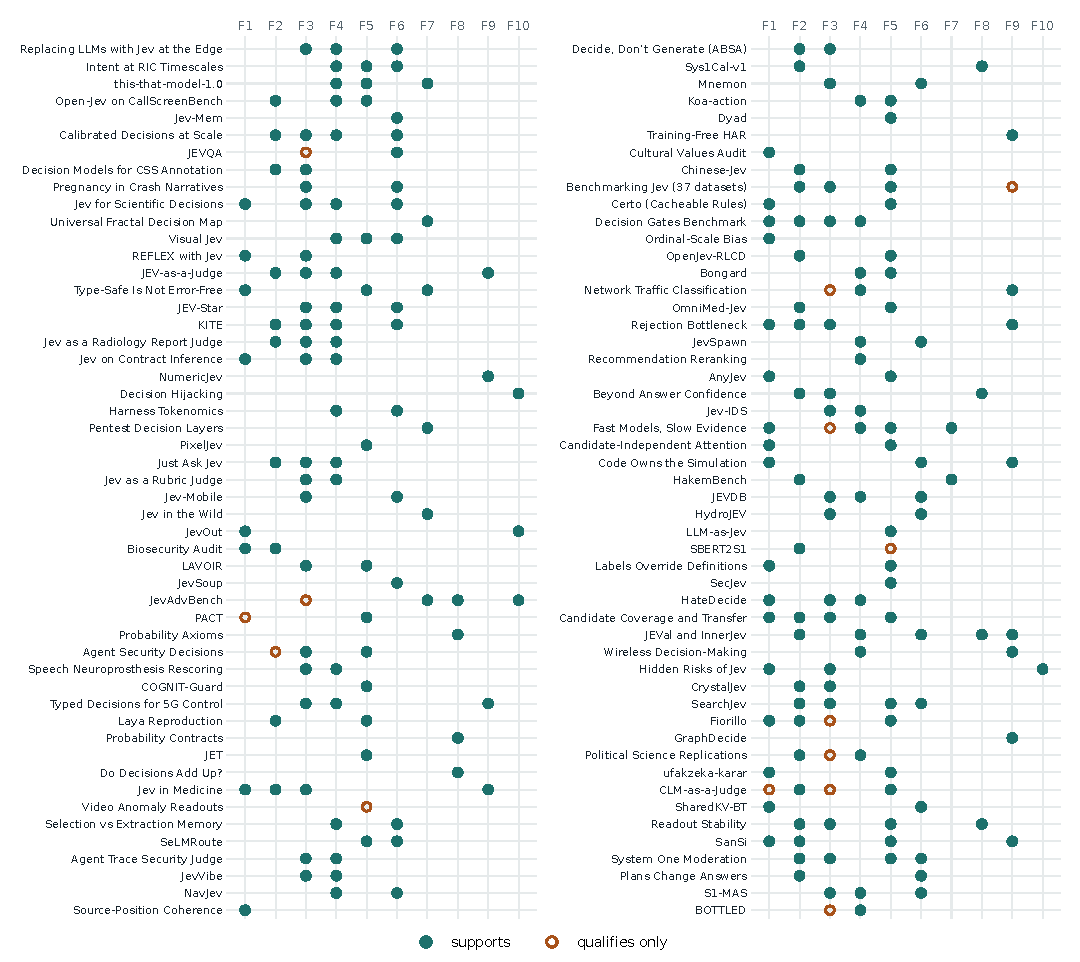
\includegraphics[width=\linewidth]{figures/matrix.pdf}
\caption{Which study bears on which finding (F1–F10, §7), derived from the evidence records (filled: supports; open: qualifies only).}\label{fig:matrix}
\end{figure}
